% !TEX root = thesis.tex

\documentclass[thesis.tex]{subfiles}

\begin{document}

\chapter{Camera Module}
\label{appendix:camera-module}

The camera module photographed from the top and side. Cardboard is used to encase the taggant and cover it from ambient lighting. Additional pieces of cardboard are used to set the smartphone to be at a fixed distance from the taggant allowing more accurate focus.

\begin{figure}[h]
\centering 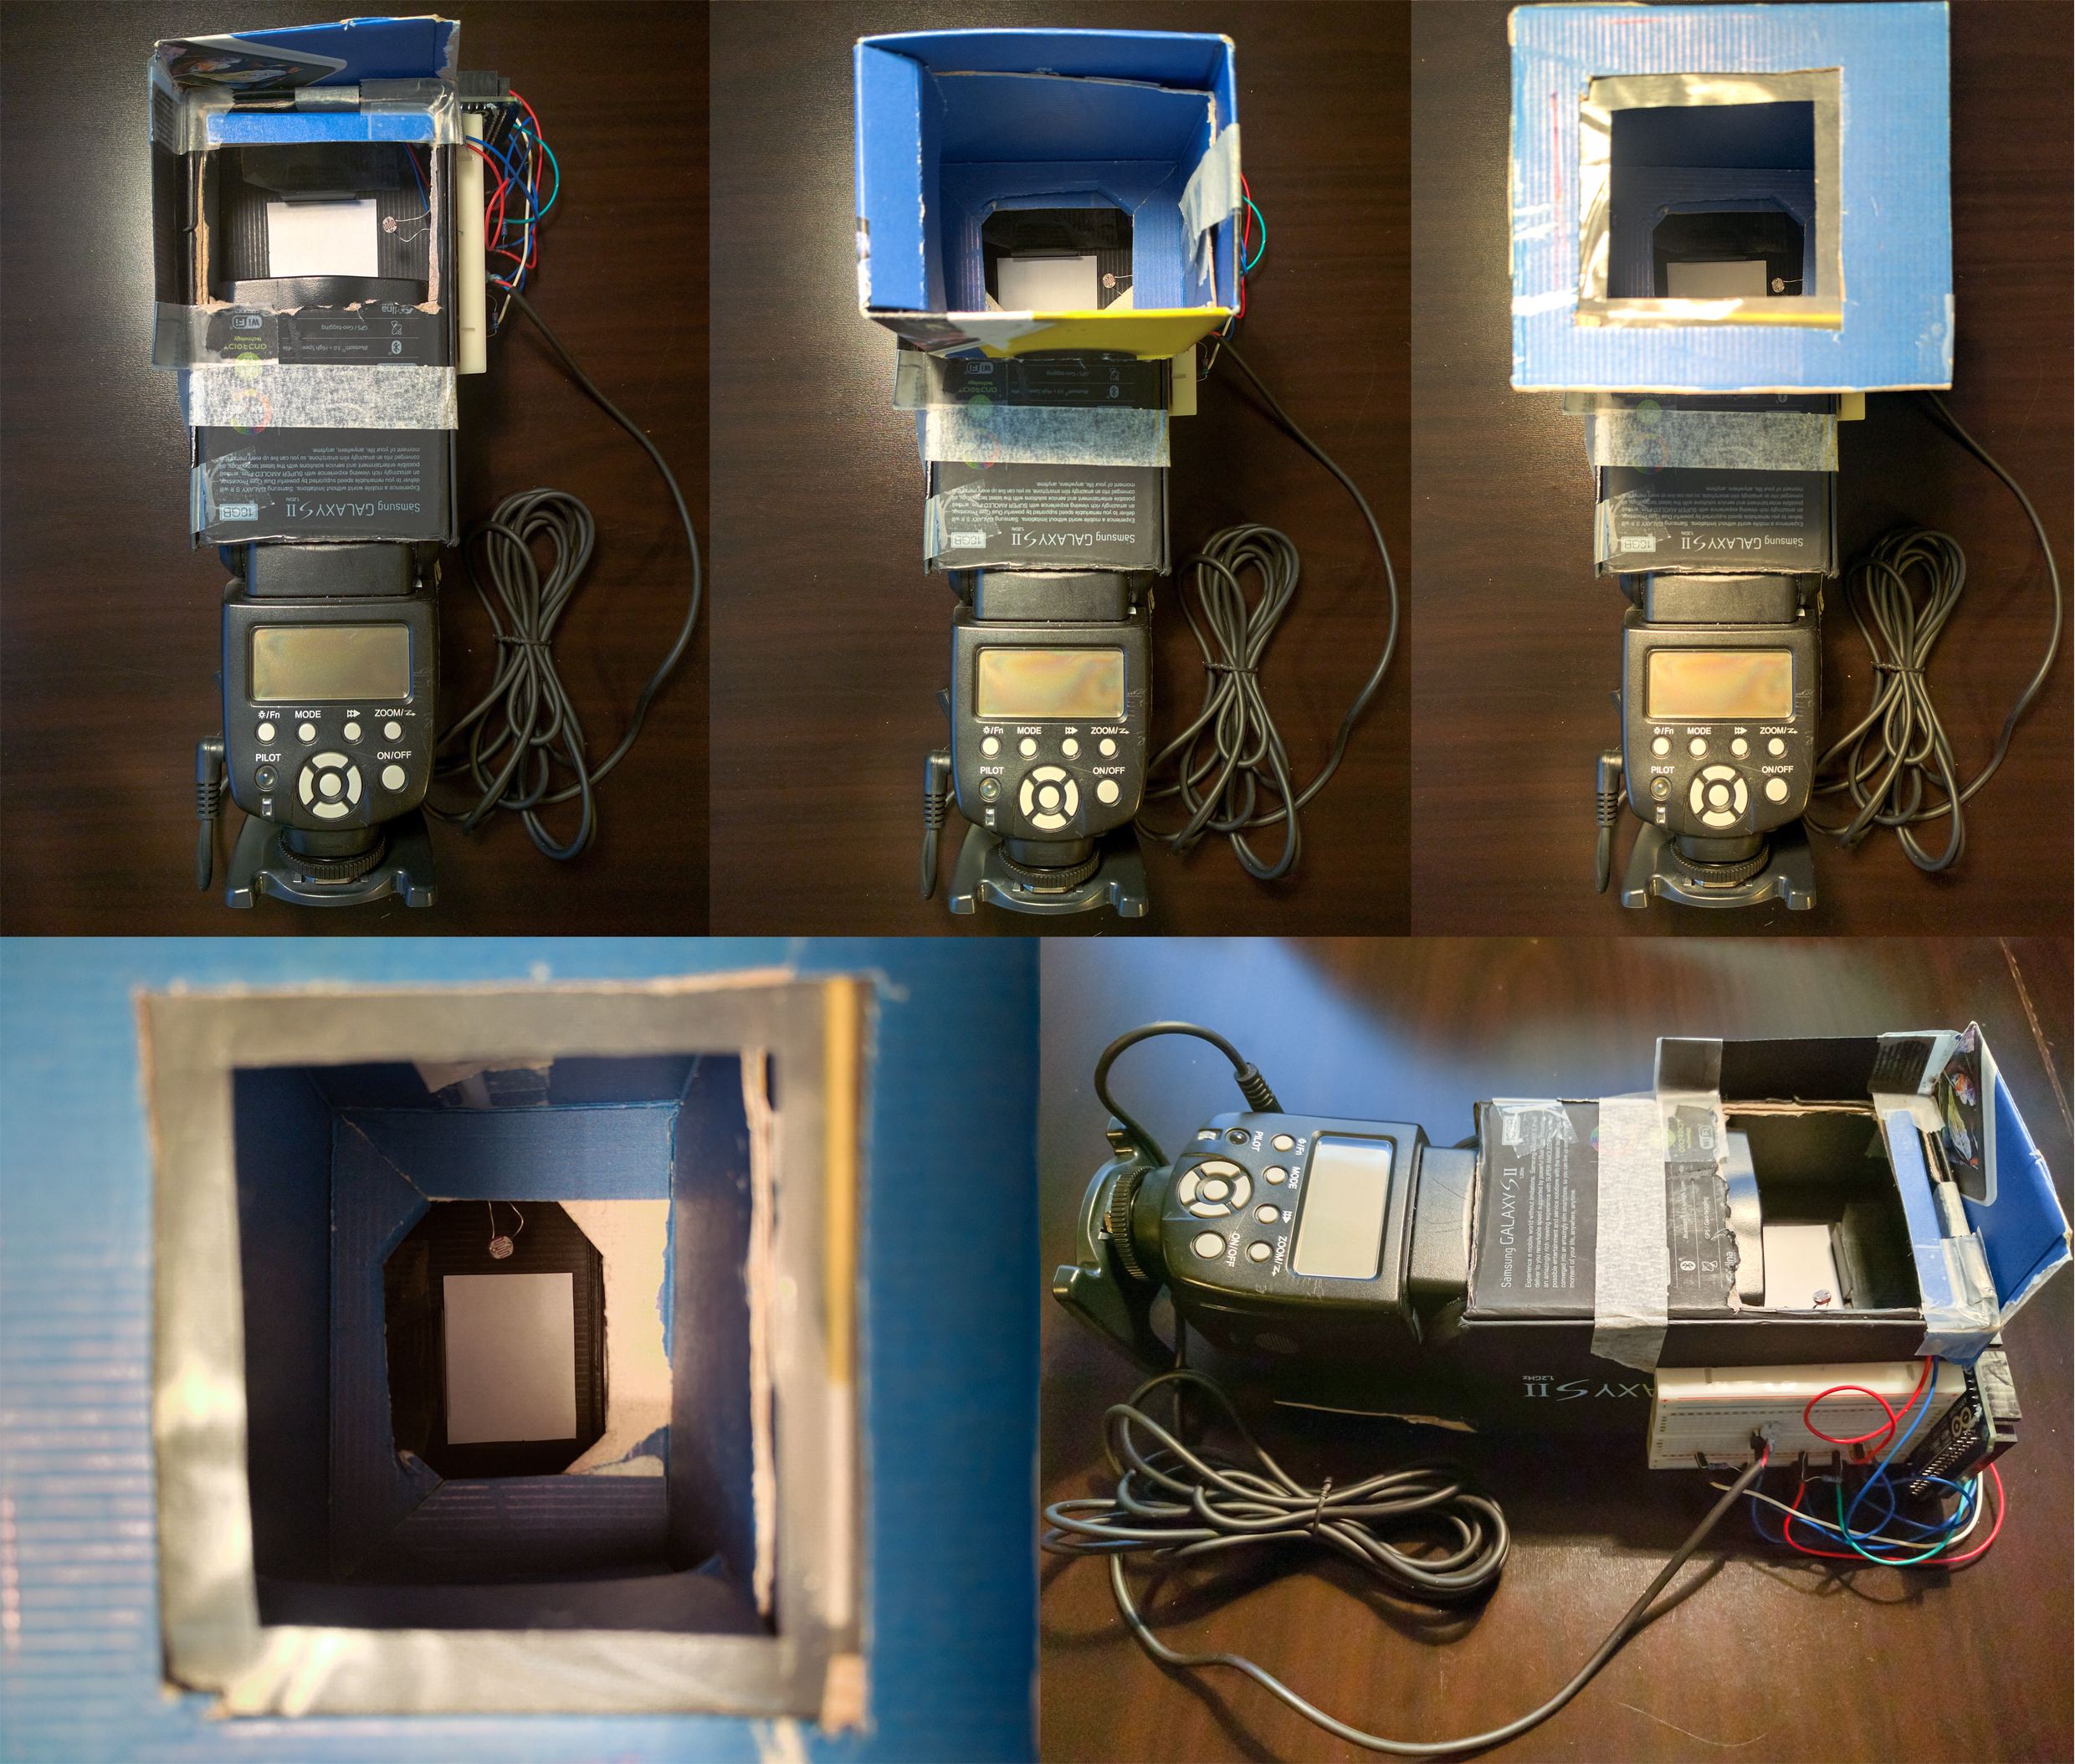
\includegraphics[width=\textwidth,height=\textheight,keepaspectratio=true]{images/design_implementation/camera_module-actual.jpg}
\end{figure}




\chapter{Microcontroller Schematics}
\label{appendix:camera-module-schematics}

The schematics for the external camera module featuring an Arduino Mega 2560 microcontroller. An optocoupler (4N35) is used to safely isolate the external light source from the rest of the circuit.

\begin{figure}[h]
\centering 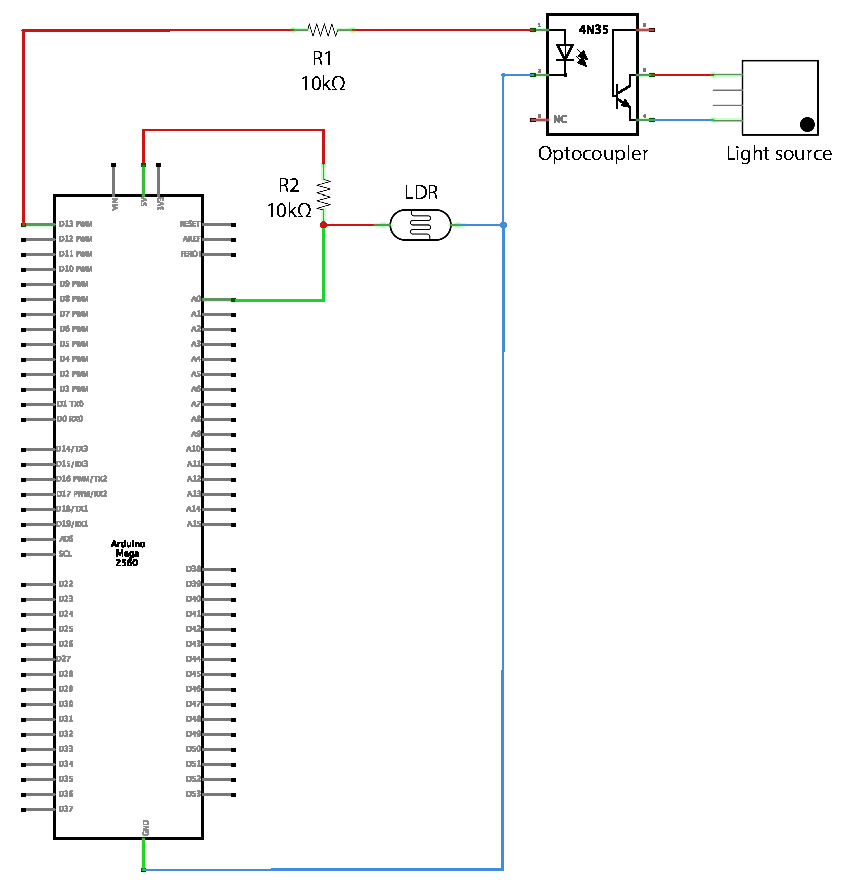
\includegraphics[width=12cm]{images/design_implementation/arduino_schematics.pdf}
\end{figure}





\chapter{Microcontroller Program (Arduino)}
\label{appendix:microcontroller-program}

The code utilizes Simon Monk's Arduino Timer library (version 1.3) \cite{arduino_timer_library}.

\lstinputlisting[language=C++,caption={main.ino}]{../app/camera-module/arduino/code/code.ino}
\clearpage
\lstinputlisting[language=C++,caption={is\_focused.ino}]{../app/camera-module/arduino/code/is_focused.ino}




\chapter{Fingerprint format}
\label{appendix:fingerprint}

The fingerprint can be represented as a $n \times m$ matrix where $n$ denotes the number of frames and $m$ the maximum number of peaks found in a single frame, and encoded as a JavaScript array with additional metadata:
\[
M=
  \begin{bmatrix}
    P_{11} & P_{12} & P_{13} \\
    P_{21} & P_{22} & 0 \\
    P_{31} & 0 & 0
  \end{bmatrix}
\]
\begin{lstlisting}[language=json,firstnumber=1]
[
  {
    timestamp: 252,
    peaks: [
      { hue: 76, intensity: 770 },
      { hue: 90, intensity: 693 },
      { hue: 60, intensity: 301 }
    ]
  },
  {
    timestamp: 844,
    peaks: [
      { hue: 74, intensity: 672 },
      { hue: 60, intensity: 310 }
    ]
  },
  {
    timestamp: 1440,
    peaks: [
      { hue: 60, intensity: 466 },
      { hue: 71, intensity: 466 }
    ]
  }
]
\end{lstlisting}


\chapter{Fingerprint Design Document}
\label{appendix:fingerprint-design-doc}
A CouchDB design document used for creating an index keyed by the peak count and weighted hue average of the first sample of each fingerprint to allow fingerprints to be queried directly by peak count and hue.
\vspace{5mm}

\lstinputlisting[language=JavaScript]{./chapters/design_doc.js}

\end{document}